\documentclass{article}
\usepackage[utf8]{inputenc}
\usepackage[a4paper,left=3.5cm,right=3.5cm,top=2cm,bottom=2cm]{geometry}
\usepackage{crop,graphicx,amsmath,array,color,amssymb,fancyhdr,lineno}
\usepackage{flushend,stfloats,amsthm,chngpage,times,,lipsum,lastpage} 
\usepackage{calc,listings,color,wrapfig,tabularx,longtable,enumitem}
\usepackage{multirow}
\usepackage{caption}
\usepackage{subcaption}
\usepackage{xcolor}
\usepackage{tcolorbox}
\definecolor{shadecolor}{rgb}{0.86,0.86,0.86}
\usepackage{float}
\usepackage{lineno}
\usepackage{csquotes}
\usepackage[italian]{babel}
\usepackage[hidelinks]{hyperref}
\usepackage{fancyhdr}
\usepackage{listings}

\title{Confronto tra Algoritmi di String Matching}
\author{Eros Pinzani}

\fancyhf{}
\fancyhead[L]{Pinzani Eros}
\fancyhead[R]{Laboratorio di Algoritmi e Strutture Dati}
\fancyfoot[C]{\thepage}
\renewcommand{\headrulewidth}{0.4pt}

\lstset{
  literate={!=}{{$\neq$}}1 {pi}{{$\pi$}}1,
  basicstyle=\ttfamily
}

\begin{document}
\pagestyle{fancy}

\begin{titlepage}
    \centering
    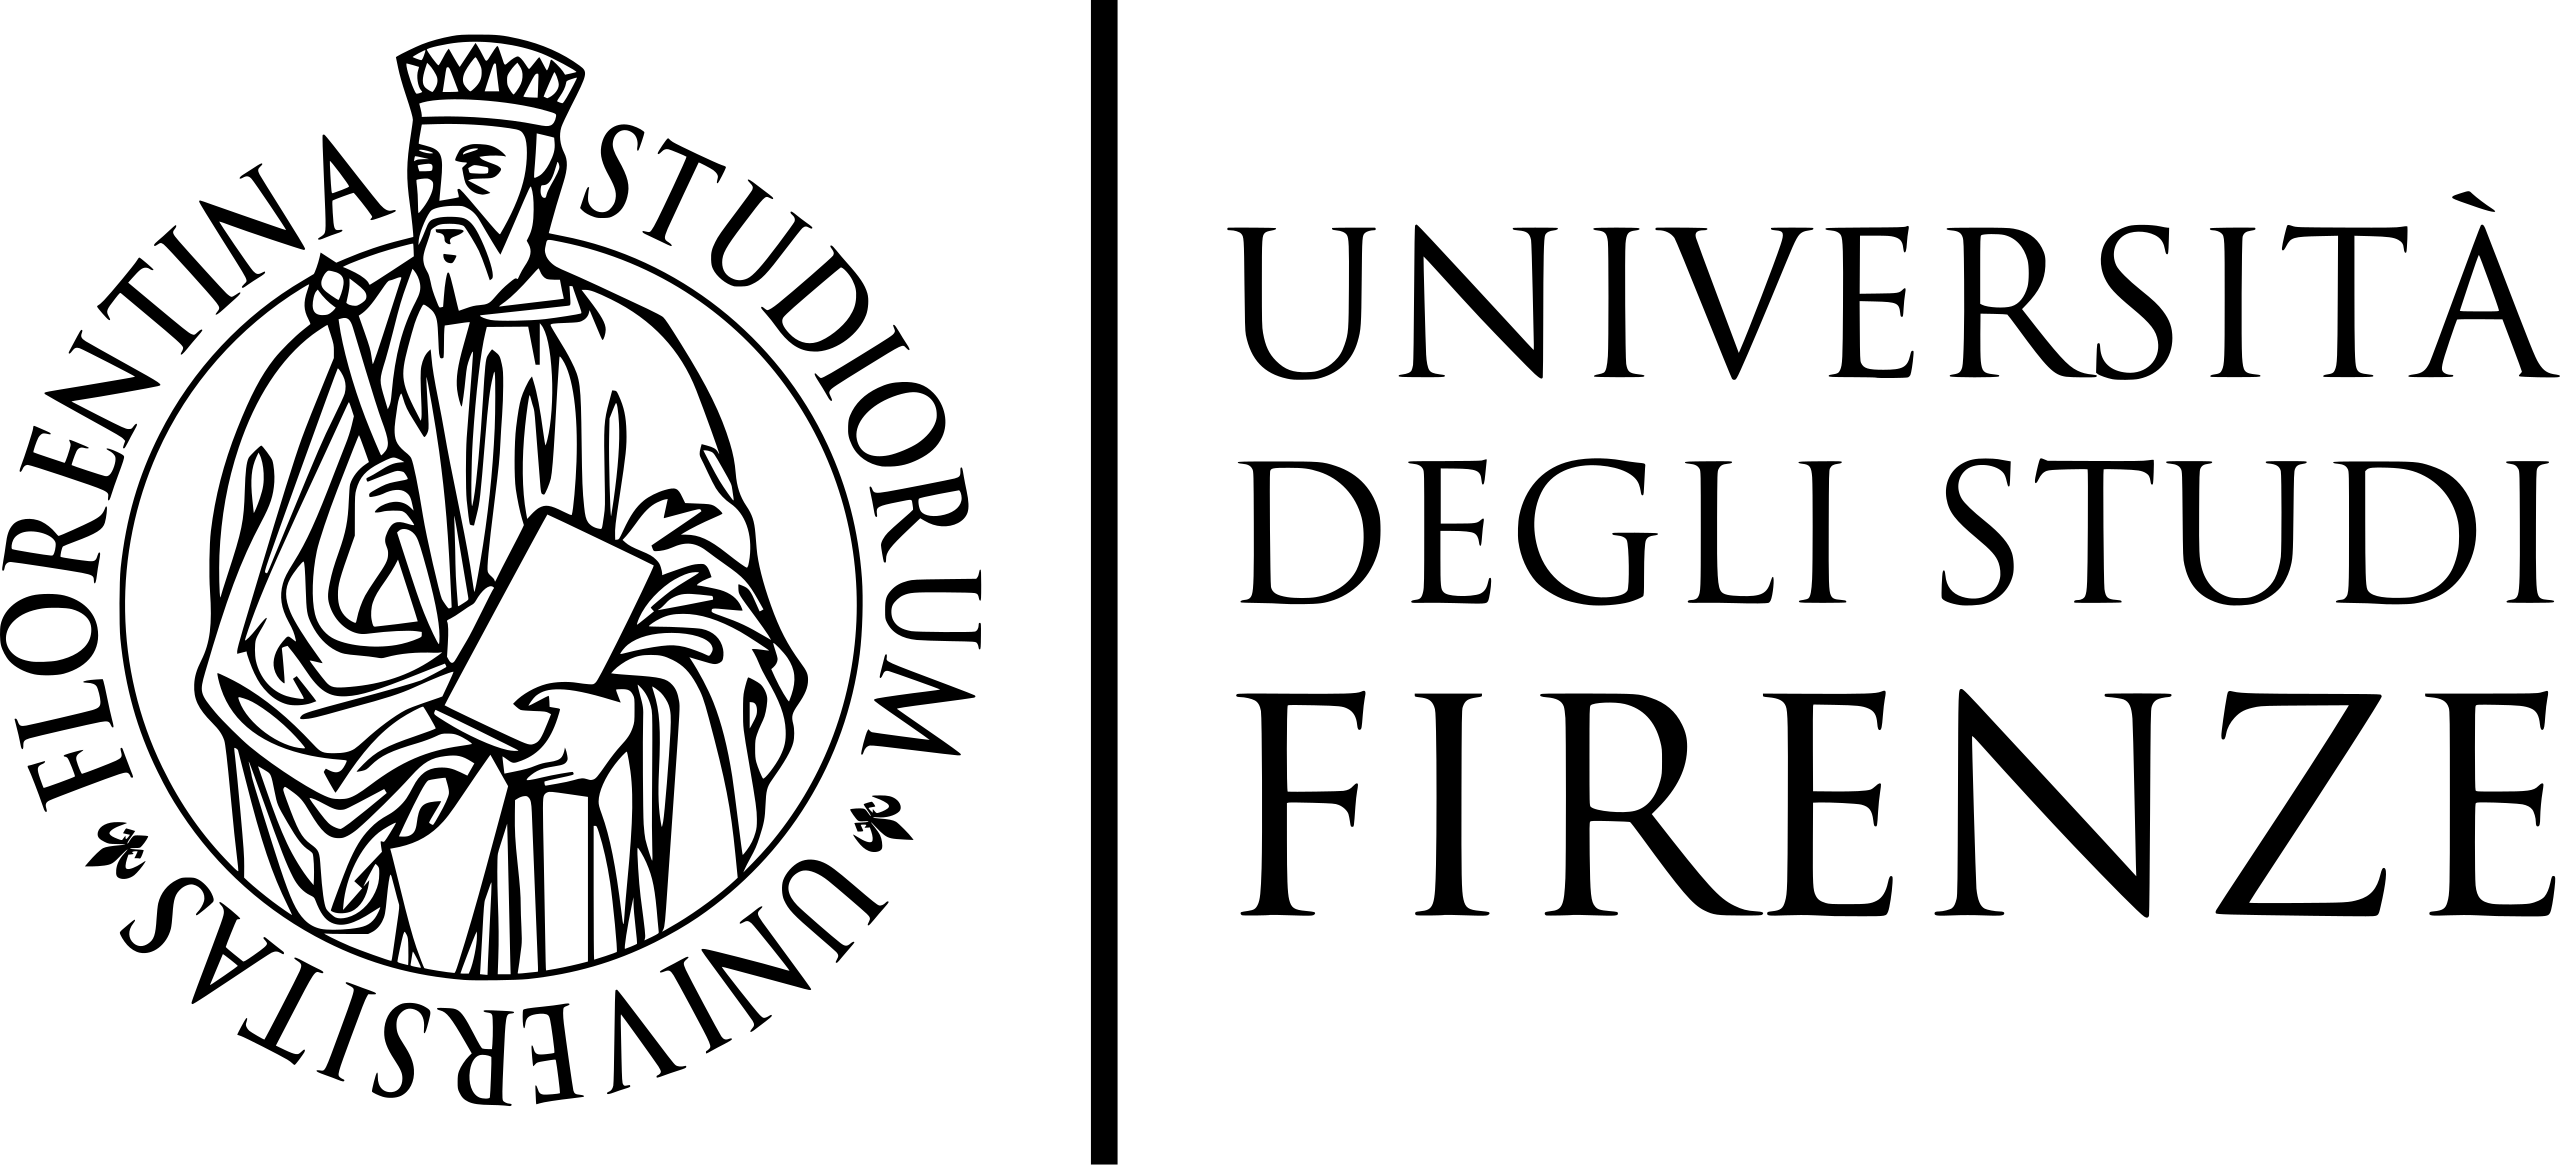
\includegraphics[width=0.90\textwidth]{img/Logo_universita_firenze.svg.png}\par\vspace{1cm}
    {\scshape\LARGE Università degli Studi di Firenze \par}
    \vspace{0.25cm}
    {\scshape\Large Dipartimento di Ingegneria dell'Informazione\par}
    \vspace{0.5cm}
    \rule{\linewidth}{0.4pt}
    \begin{center}
        {\Huge{\bfseries \textbf{Confronto tra Algoritmi di String Matching}\par}}
    \end{center}
    \rule{\linewidth}{0.4pt}
    \vspace{1cm}

    \begin{minipage}[t]{0.4\textwidth}
        \begin{flushleft} \large
            \emph{Autore:}\par
            Eros Pinzani\par
        \end{flushleft}

        \begin{flushleft} \large
            \emph{N° Matricola:}\par
            7030989\par
        \end{flushleft}
    \end{minipage}
    \hfill
    \begin{minipage}[t]{0.4\textwidth}
        \begin{flushleft} \large\raggedleft
            \emph{Corso:}\par
            Algoritmi e Strutture Dati
        \end{flushleft}

        \begin{flushleft} \large\raggedleft
            \emph{Docente corso:}\par
            Simone Marinai\par
        \end{flushleft}
    \end{minipage}

\end{titlepage}

\newpage
\renewcommand{\contentsname}{Indice}
\tableofcontents
\pagenumbering{arabic}
\newpage
\section{Introduzione generale}
\subsection{Breve descrizione dello svolgimento degli esercizi}
Per ogni esercizio suddividiamo la sua descrizione in 4 parti fondamentali:

\begin{itemize}
    \item \textbf{Spiegazione teorica del problema} : qui è dove si descrive il problema che andremo ad affrontare in modo teorico partendo dagli assunti del libro di Algoritmi e Strutture Dati e da altre fonti.
    \item \textbf{Documentazione del codice} : in questa parte spieghiamo come il codice dell'esercizio viene implementato.
    \item \textbf{Descrizione degli esperimenti condotti} : partendo dal codice ed effettuando misurazioni varie cerchiamo di verificare le ipotesi teoriche.
    \item \textbf{Analisi dei risultati sperimentali} : dopo aver svolto i vari esperimenti riflettiamo sui vari risultati ed esponiamo una tesi.
\end{itemize}

\subsection{Specifiche della piattaforma di test}
La piattaforma di test sarà la stessa per ogni esercizio che vedremo. Partiamo dall'hardware del computer fondamentale da conoscere per questo esercizio:

\begin{itemize}
    \item \textbf{CPU} : AMD Ryzen™ 5 PRO 7540U (da 3,2 GHz fino a 4,9 GHz)
    \item \textbf{RAM} : 16 GB LPDDR5X-6.400MT/s
    \item \textbf{SSD} : 512 GB M.2 2280 PCIe Gen4 TLC Opal
\end{itemize}

Il linguaggio di programmazione utilizzato sarà Python e la piattaforma in cui il codice è stato scritto e 'girato' è l'IDE \textbf{Visual Studio Code}. La stesura di questo testo è avvenuta tramite l'utilizzo di \textbf{Visual Studio Code} e opportune estensioni.

\newpage

\part{Algoritmo ``ingenuo'' vs Algoritmo KMP}

\begin{tcolorbox}[colback=lightgray!20,
        colframe=black,
        arc=3mm, auto outer arc,]

    \textbf{Esercizio A}
    \begin{itemize}
        \item Vogliamo confrontare gli algoritmi ``ingenuo'' e KMP per effettuare string matching
        \item Per fare questo dovremo:
              \begin{itemize}
                  \item Scrivere i programmi Python che:
                        \begin{itemize}
                            \item implementino quanto richiesto
                            \item eseguono un insieme di test che ci permettano di comprendere vantaggi e svantaggi delle diverse implementazioni
                        \end{itemize}
                  \item Svolgere ed analizzare opportuni esperimenti
                  \item Scrivere una relazione che descriva quanto fatto
              \end{itemize}
    \end{itemize}
\end{tcolorbox}

\section{Spiegazione teorica del problema }

\subsection{Introduzione}
Nella seguente parte della relazione viene descritta l'implementazione degli algoritmi di string matching ``\textbf{ingenuo}'' e \textbf{Knuth-Morris-Pratt}, d'ora in poi chiamato \textbf{KMP} per semplicità. Questi algoritmi permettono di ricercare una data stringa, chiamata \textbf{pattern}, all'interno di un \textbf{testo} più o meno complesso. Verranno quindi messi a confronto i due algoritmi per valutarne la complessità in termini di tempo necessario e numero di confronti effettuati prima di trovare tutte quante le occorrenze.

\subsection{Cos'è un algoritmo di string matching?}
Gli algoritmi di string matching sono algoritmi che permettono di trovare una o più occorrenze di una stringa, chiamata \textbf{pattern}, all'interno di un'altra stringa, chiamata \textbf{testo}. Questi algoritmi sono utilizzati in molti campi, ad esempio nella ricerca di pattern in sequenze di DNA oppure vengono utilizzati da motori di ricerca per individuare pagine web pertinenti alle query.
Andiamo ora ad analizzare nel dettagli gli algoritmi ``\textbf{ingenuo}'' e \textbf{KMP} osservando che a parità di occorrenze del pattern trovate il secondo algoritmo risulta essere più efficiente del primo.

\subsubsection{Algoritmo ``ingenuo''}
L'algoritmo ``\textbf{ingenuo}'' è il più semplice da implementare e consiste nel confrontare il pattern con ogni sottostringa del testo di lunghezza uguale al pattern. In questo modo, l'algoritmo scorre il testo e per ogni posizione confronta il pattern con la sottostringa del testo. Se i caratteri corrispondono, l'algoritmo continua a confrontare i caratteri successivi fino a quando non trova una occorrenza completa o un carattere diverso. In caso di occorrenza completa, l'algoritmo registra la posizione in cui è stata trovata la occorrenza.
\begin{itemize}
    \item Pseudocodice:
        \begin{verbatim}
        NAIVE-STRING-MATCHER(T, P)
            n = T.length
            m = P.length
            for s = 0 to n - m
                if P[1...m] == T[s + 1...s + m]
                    stampa "Occorrenza del pattern con spostamento s"
        \end{verbatim}
    \item Descrizione dell'algoritmo:
          \begin{enumerate}
              \item L'algoritmo inizia salvando le lunghezze del testo e del pattern nelle rispettive variabili \textit{n} e \textit{m}.
              \item Successivamente, inizia un ciclo che scorre il testo da 0 a \textit{n} - \textit{m}
              \item Quindi confronta tutto il pattern con la sottostringa del testo di lunghezza \textit{m} a partire dalla posizione \textit{s}.
              \item Se la condizione viene rispettata allora viene stampata la posizione \textit{s} in cui è stata trovata l'occorrenza.
          \end{enumerate}
    \item Implementazione:
          \begin{figure}[H]
          \centering
          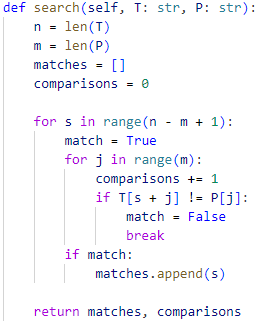
\includegraphics[width=0.4\textwidth]{img/Naive_search.png}
          \caption{Implementazione Python dell'algoritmo ``ingenuo''}
          \label{fig:naive-implementation}
      \end{figure}
    \item Motivazioni per l'uso dell'algoritmo ``ingenuo'':
          \begin{itemize}
              \item Semplicità di implementazione
              \item Efficace per casi semplici e non ripetitivi
              \item Nessuna pre-elaborazione del pattern
              \item Basso consumo di memoria
          \end{itemize}
\end{itemize}

\subsubsection{Algoritmo KMP}
L'algoritmo \textbf{KMP} è un algoritmo di string matching più avanzato rispetto a quello ``\textbf{ingenuo}'' che evita confronti ridondanti. Attraverso una fase preliminare in cui viene analizzato il pattern l'algoritmo costruisce una struttura ausiliaria chiamata \textbf{funzione prefisso $\pi$} grazie alla quale, durante la fase di ricerca, in caso di discordanza tra pattern e testo, permette di saltare alcuni confronti inutili e determinare il punto da cui continuare la ricerca.\\
La funzione prefisso $\pi$ associa ad ogni posizione \textit{i} del pattern il numero massimo di caratteri iniziali (prefisso) che coincidono con un suffisso della sottostringa del pattern P[1...\textit{i}]. Ovvero, $\pi[i]$ rappresenta la lunghezza del più lungo prefisso del pattern che è anche un suffisso di P[1...\textit{i}]. È grazie a questa funzione che l'algoritmo stabilisce di quanto può essere traslato in avanti il pattern, continuando a mantenere allineati i caratteri già confrontati.
\begin{itemize}
    \item Pseudocodice:
        \begin{lstlisting}
        COMPUTE-PREFIX-FUNCTION(P)
            m = P.length
            Sia pi[1...m]$ un nuovo array
            pi[1] = 0
            k = 0
            for q = 2 to m
                while k > 0 and P[k + 1] != P[q]
                    k = pi[k]
                if P[k + 1] == P[q]
                    k = k + 1
                pi[q] = k
            return pi
        \end{lstlisting}
    \item Descrizione dell'algoritmo:
          \begin{enumerate}
              \item 
          \end{enumerate}
    \item Implementazione:
          \begin{figure}[H]
          \centering
          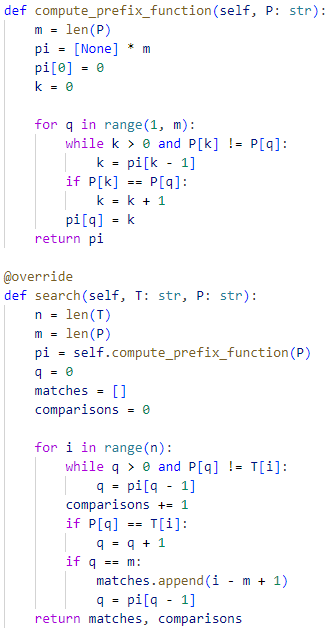
\includegraphics[width=0.4\textwidth]{img/KMP_search.png}
          \caption{Implementazione Python dell'algoritmo KMP}
          \label{fig:KMP-implementation}
      \end{figure}
    \item Motivazioni per l'uso dell'algoritmo KMP:
          \begin{itemize}
              \item 
          \end{itemize}
\end{itemize}

\end{document}